\documentclass[MSc]{icldt}

\usepackage{graphicx}
\usepackage[T1]{fontenc}
\usepackage[scaled]{beramono}
\usepackage{amssymb}


\usepackage{color}
\definecolor{bluekeywords}{rgb}{0.13,0.13,1}
\definecolor{greencomments}{rgb}{0,0.5,0}
\definecolor{redstrings}{rgb}{0.9,0,0}

\usepackage{algorithm}
\usepackage{algorithmic}

\usepackage{listings}
\lstset{language=C,
showspaces=false,
showtabs=false,
breaklines=true,
showstringspaces=false,
breakatwhitespace=true,
escapeinside={(*@}{@*)},
commentstyle=\color{greencomments},
keywordstyle=\color{bluekeywords}\bfseries,
stringstyle=\color{redstrings},
basicstyle=\ttfamily
}

%%Change caption name in code snippets
%\renewcommand*{\lstlistingname}{Code}

\title{Sampling in a Large Network\\Background Report}
\author{Xenofon Foukas}
\date{}
% Please specify you department here.
\department{Computing}
% The college regulations do not require that you mention 
% your supervisor on the titlepage of you dissertation.
% If you want to do so put her name here.
%\supervisor{Alexander Wolf}
% The college regulations do neither require nor forbid 
% a dedication of your dissertation to somebody or something. 
% If you want to include a dedication put the text here. 
\dedication{}
\college{Imperial College London}
\field{Advanced Computing}
\setlength{\topmargin}{0in}
\setlength{\headheight}{0in}
\setlength{\headsep}{0in}

\setlength{\textwidth}{6.5in}
\setlength{\oddsidemargin}{-0.12in}
\setlength{\evensidemargin}{-0.12in}

\begin{document}

\maketitle

%\section*{Acknowledgments}

\tableofcontents
\chapter{Introduction}

\section{Motivation}


It is very often beneficial to architect networks and overlays as fully decentralized systems rather than choosing a centralized architectural approach. Such a solution is usually more reliable and resilient to failures, while it can offer high performance with a relatively small cost. Moreover, no component has a complete view or control over the whole network when performing usual computations like packet routing and searching for specific key-value pairs, where only local information are being used, resulting in a more flexible and secure model. A very common and well known example of a decentralized solution are peer-to-peer networks, where nodes communicate with each other sharing their resources (e.g. processing power, memory etc). Such networks are very common and can often reach a size of thousands or millions of nodes (e.g. BitTorrent and Tor).

Regardless of the benefits that such an approach offers, it is very often necessary to compute global properties of the network, which are required for performing some important tasks, like maintenance and routing. Some typical examples of global properties are the size of the network and its mixing time, i.e. the number of hops after which a random walk approaches the network's stationary distribution and becomes independent of the starting point. Computing these properties using either centralized or decentralized algorithms is generally a feasible task. However, the real challenge is finding a solution that can be efficient both in terms of time and communication cost.


There exist many proposals for efficient computation of global parameters in decentralized systems, each following different approaches, from sampling and projecting local properties to computing aggregates of data distributed over the network. Some algorithms are based on deriving useful properties from the spectrum of the network by computing the most significant eigenvalues of some descriptive matrix. There has been a proposal of a particularly interesting fully decentralized algorithm \cite{6195806} that can compute efficiently some global properties like the mixing time, by using the eigenvalues of a matrix related to the adjacency matrix of the network. While this algorithm appears to have good results in a simulation environment it has not been tested using some concrete implementation. Additionally, the estimates it provides are lacking accuracy in networks with high churn rates. Thus, it would be interesting to better investigate the algorithm's potential and to try and improve its weaknesses.


\section{Contributions}

In this project we try to design and implement a protocol based on the aforementioned algorithm. Such a protocol should be able to efficiently perform the tasks required by the algorithm and it should be designed in a way that allows its deployment into common network and overlay topologies, e.g. a Chord or Pastry topology. In addition, the project should attempt to enhance the proposed algorithm's robustness for better estimations in networks with high churn rates. This enhancement is important, since it will allow the algorithm to be applied in more networks. For instance most common peer-to-peer networks are by nature highly unstable, since nodes continuously join and depart from the network, altering its properties.

This project presents both theoretical and practical issues that need to be addressed in an elegant and efficient way. The nature of the project presents us with two main challenges. The first challenge is to design a protocol that is robust and efficient while it remains simple and to implement it with extensibility in mind, both in functionality and in compliance with a variety of underlying network communication protocols. The second challenge is that such a protocol should be evaluated in an environment that closely resembles a real large-scale network. This will allow us to better determine its applicability and usefulness in real-life scenarios.


\section{Report Structure}

We begin by making a short introduction on decentralized networks, presenting techniques and related work in computing global properties of networks and overlays in Chapter \ref{sec:background}. We also present in greater depth the decentralized algorithm that will be the basis of our proposed protocol, discussing its evaluation results and its limitations.

In Chapter \ref{sec:design} we present the design requirements that our proposed protocol should fulfill, discussing both advantages and disadvantages that certain design decisions might incur to the applicability and efficiency of our proposal. Moreover, we attempt to present a general design overview of the proposed protocol.

Finally, in Chapter \ref{sec:progress} we briefly discuss some of the goals that we would ideally want to achieve during the next few months and the stages in which we plan on doing this.



\chapter{Background}
\label{sec:background}

This chapter makes a short introduction on decentralized networks and presents techniques and related work in computing global properties of networks and overlays, as it is important to create a solid context that better explains the motivation of our work. Furthermore, this section makes a detailed presentation of the decentralized algorithm that will be the basis of our proposed protocol.



\section{Decentralized Networks}

A decentralized network is generally a network in which at least some of the processing is done at individual nodes and information is shared by and often stored at the nodes \cite{parker2003mcgraw}. In such a network participants are able to join or leave at any time. One of the best and most common examples of a decentralized network are peer-to-peer systems. Such a system is essentially a network of applications, partitioning resources like processing power and disk storage and balancing work loads amongst peers. The whole partitioning process is performed directly by the network participants without the intervention of servers providing some sort of central coordination. Typically each peer maintains only a local view of the network that is limited to information regarding neighboring nodes. Some major advantages of peer-to-peer networks and generally of any decentralized network is their resiliency to failures due to the removal of a central point of coordination and control and the high performance/price ratio that they offer. However, due to the limited view that each node has for the global state of the network, discovering properties like the size and the diameter of the network, is considered a more challenging task that usually requires the cooperation of all the participating nodes. Additionally it is often the case that sophisticated mechanisms are required to deal with the continuous topological changes that decentralized systems present, due to the addition and removal of nodes.

There is a large number of decentralized networks used in practice. A typical example are systems that use a distributed hash table (DHT) to provide a lookup service of key-value pairs that is similar to a simple hash table, only spreading the pairs over nodes in the network based on some properties of both the nodes and the keys, essentially creating an overlay network on top of the physical. Chord \cite{Stoica:2001:CSP:964723.383071} and Pastry \cite{Rowstron:2001:PSD:646591.697650} are two commonly used protocols that implement such DHT systems. 

\section{Related Work}

In large scale decentralized networks there is often a need to know global state properties in order to deal with issues like maintenance, routing and quality of service. There has been a lot of research on computing global properties that can be broadly divided into three major categories; aggregation, sampling and spectral computation algorithms.

\subsection{Aggregation Algorithms}

Aggregation acts as a summarizing mechanism of the overall state within the network. Each participating node shares some local information in the form of numerical values, that when combined can be used to infer global information for the system, which in turn can provide indicators to evaluate global properties. These indicators are very often desirable, since they can provide useful hints when attempting to ensure some level of performance, QoS etc \cite{Makhloufi:2009:DAP:1692742.1692756}. Aggregation techniques can vary, from using simple aggregate functions (sum, max, average etc.) to more advanced like histograms [citation] and linear projections [citation]. Aggregation protocols can be further divided into two subcategories; gossip-based and tree-based aggregation schemes \cite{Makhloufi:2009:DAP:1692742.1692756}.

Gossip algorithms operate in an analogy to how gossip news spread in a social network. Nodes form pairs and exchange their information, spreading them to the hole network. Depending on the probability distribution used by a node to choose its pair, we can divide them in uniform \cite{Kempe:2003:GCA:946243.946317} and non-uniform \cite{Kempe:2004:SGR:1039488.1039491} \cite{Rabbat:2007:SGA:1524876.1525177}. A fundamental uniform gossip-based algorithm proposed by Kempe et al. is \textit{Push-Sum} \cite{Kempe:2004:SGR:1039488.1039491}, where each node begins with a local value $x_v$ and tries to compute some estimations like the average $1/n \sum{x_v}$. A non-uniform aggregation algorithm is \textit{Spatial gossip} \cite{Kempe:2004:SGR:1039488.1039491} \cite{Rabbat:2007:SGA:1524876.1525177}, where the selection of the nodes is done according to their distance. Due to the nature of gossip-based algorithms, they usually are simple, scalable and failure-resistant. However, every node needs to exchange and aggregate a large amount of data, resulting in high computation and communication costs.

Tree-based algorithms compute aggregates by using trees in a bottom-up fashion. Usually a node that initiates the protocol makes a request to build a spanning tree on the network (e.g. by using BFS) and then aggregate values are computed and propagated to the higher levels of the tree. Some well-known tree-based algorithms are \textit{SingleTree} \cite{Bawa03estimatingaggregates} and \textit{GAP} \cite{Dam05ageneric}. This type of aggregation algorithms have lower communication costs compared to gossip-based, since data are only propagated from lower levels of the tree to higher ones. However, they are more sensitive to failures, due to the fact that data exchanges depend on a spanning tree, which will usually require reconstruction after a node crashes.

\subsection{Sampling Algorithms}

In this category we find algorithms that try to infer global network properties by performing projections in local properties acquired by using sampling techniques. Some well-known techniques, used for estimating the size of the network are \textit{Random Tour} and \textit{Sample and Collide} \cite{Massoulie:2006:PCS:1146381.1146402}. The former achieves this by performing a random tour at the network and by keeping track of the number of nodes visited. The average number of hops before returning to the original node, also called hitting time, is related to the global probability of visiting that node and can be computed locally. Using these information, the size of the network can be estimated. The latter technique is based on the birthday paradox, i.e. if 23 people are found in the same room, there is a 50\% probability that two of them have birthday at the same day. Using this property, the algorithm randomly samples network nodes and keeps track of the number of samples acquired before a collision is recorded. Then, by using the number of sampled nodes and the birthday paradox property, an estimation of the network size is possible.


\subsection{Spectral Computation Algorithms }

While the algorithms presented in the previous sections can be very useful and in most cases can be easily implemented, the information they provide us are network independent and they do not map properties related to the structure and the connectivity of the network \cite{6195806}. The algorithms of this category can achieve this by analyzing the spectrum of the network graph. The general idea behind all spectral algorithms is that they attempt to compute the eigenvalues of a matrix describing or being somehow related to the structural properties of the network, which is distributed among the network's nodes. In this category belong algorithms like the one proposed by Kempe and McSherry or EigenSpeed and EigenTrust \cite{Kempe:2004:DAS:1007352.1007438} \cite{Kamvar:2003:EAR:775152.775242} \cite{Snader:2009:ESP:1855663.1855672}. The decentralized algorithm used as the basis of our protocol also belongs in this category.


\section{A Decentralized Algorithm for Estimation of Global Properties}

The intuition behind this decentralized algorithm is that each node in the network can compute the impulse response of a linear dynamic system, for which the state-transformation matrix is a descriptive matrix of the network derived by the network graph, i.e. it is closely related to its adjacency matrix. Before proceeding with the algorithm's overview, it would be useful to further analyze the context of this algorithm as well as its goal.

The impulse response of a dynamic system is the output it produces when it is presented with some input signal, called an \textit{impulse}. In the case of a network, an impulse could be a value that a node received resulting in a transformation to a new state that has some output, which can be viewed as the impulse response. For the whole system, the aforementioned action and reaction could be described by the system of equations:

\begin{equation}
\label{eq:one}
x(t+1) = Ax(t)+Bu(t)
\end{equation}  
\begin{equation}
\label{eq:two}
y(t)=Cx(t)
\end{equation}  

where $x(t) \in \mathbb{R}^n$ is the state of a network of size $n$, $u(t) \in \mathbb{R}$ is the input and $y(t) \in \mathbb{R}$ is the output at some time $t$. $A \in \mathbb{R}^{n \times n} $ is the state-transformation matrix and $B, C \in \mathbb{R}^n$ are vectors used for mapping the input to the state of the system and the state to the output respectively. For the decentralized algorithm to be applicable, $A$ should be any matrix related to the adjacency matrix of the network that can be produced using only local information (e.g. a transition matrix). Thus, a requirement of $A$ is that $a_{uv} \neq 0$ iff $u=v$ or there is an edge from $v$ to $u$ (it must be noted that for this algorithm the adjacency information need to be presented column-wise). Initially, the system is in the quiescent state, i.e. $x(0)=0$. We can denote the impulse response with $h(t)$ and using the above equations we can define it as $h(t)=CA^{t-1}B$, by using as input $u(0)=1$ and $u(t)=0$ for $t > 0$.

It can be easily seen that each network node would require only local information and the inputs it receives by its neighbors in order to compute the impulse responses at any time $t>0$. The algorithm is based on the idea that through the impulse responses gathered over some time period, we can make an estimation of the spectrum of matrix $A$ (i.e. compute its dominant eigenvalues). Moreover, if this time period is long enough, the algorithm is exact. However, even in a short number of rounds, the estimation could be close to the exact solution if the diameter of the network is very low compared to the size of the network, an assumption reasonable for most peer-to-peer networks.

\subsection{Algorithm Overview}

The steps required can be seen in Algorithm \ref{alg:basic}. Each node $v$ holds one column $a_v$ of matrix $A$, containing the local information related to the adjacency matrix.

\begin{algorithm}
\caption{estimation algorithm at node $v$}
\label{alg:basic}
\begin{algorithmic}[1]

\STATE $x_v \leftarrow$  Choose a value uniformly from $\{0,1\}$
\STATE $h_v(1) \leftarrow x_v$
\FOR{$t \leftarrow 2 \dots k$}

\FOR{$u \in$ out-neighbours$(v)$} 

\STATE send value $x_{v}a_{uv}$ to $u$
\STATE collect all values $w$ sent by in-neighbors
\STATE $x_v \leftarrow \sum{w}$
\STATE $h_v(t) \leftarrow x_v$

\ENDFOR

\ENDFOR
\STATE $\hat{A_v} = $ Kung's realization with $h_v(1),\dots, h_v(k)$
\STATE compute the dominant eigenvalues of $\hat{A_v}$
\STATE exchange the eigenvalues with neighbors
\STATE collect estimates from neighbors
\STATE adjust estimates to the median of the collected estimates

\end{algorithmic}
\end{algorithm}

In the beginning each node must randomly select a value from 0 or 1 as the initial input. At each of the following rounds, every node computes locally $x_v a_{uv}$ and sends it to all its out-neighbors. Then, every node computes a new $x_v$ by adding the values received by the in-neighbors and stores this value as the impulse response $h_v$ of this round. 

As already stated, every node holds only partial information of matrix $A$. However to analyze it's spectrum, the whole matrix is required. Using the impulse responses gathered in the previous phase, $A$ or an approximation of $A$ can be computed by using an approximation of Kung's realization algorithm \cite{1992040} \cite{1164997}. A realization algorithm is a system identification technique that can generate a system realization by using impulse response data. What this means is that given the impulse responses of the system we can compute approximations of the matrix and vectors presented in Equations (\ref{eq:one}), (\ref{eq:two}). A divergence of this algorithm compared to Kung's is that the latter requires at least $k=2n-1$ steps, where $n$ would be the size of the network, while this algorithm requires a $k$ that is only on the order of the network's diameter. Using the approximation $A_v$ of matrix $A$ computed in this step, we can then proceed and find its dominant eigenvalues. An additional step that can further improve the results of the algorithm is for neighboring nodes to exchange their estimations and adjust them to the median of the available values, following a gossip style method.

\subsection{Evaluation results and Limitations}

This algorithm was evaluated in a simulated environment for various types of networks and overlays (e.g. Chord). The main evaluation criterion was the mixing time of the network that was computed using the second eigenvalue modulus of $A_v$. The mixing time is the necessary length of a random walk required to compute the steady state probabilities of the network. In general, the algorithm performs well producing accurate estimates of the mixing time, when no failures occur. However, in unstable networks, where even one failure occurred, the results of the evaluation revealed large errors in some cases. Thus the current algorithm is more applicable to stable networks.  



\chapter{Protocol Design}
\label{sec:design}

In this chapter we present the design requirements that our proposed protocol should fulfill, discussing advantages and disadvantages that certain design decisions might incur to the applicability and efficiency of our proposal. Moreover we attempt to present a general design overview of our proposal.

\section{Design Requirements}

Before designing a protocol for computing global network properties, it is important to analyze the requirements that such a protocol should satisfy. This will help us to better confine our problem and mark some goals that a probable solution will need to achieve. There has been a wide analysis of requirements for protocols and decentralized systems \cite{Rose01onthe} \cite{Kendall:1994:NDC:974938}. Those that are most important in our case are presented below:


\subsubsection*{Correctness}

The protocol should yield correct results. That is, the exchange of control messages and matrix components should lead to the computation of estimation values for the global properties, that closely resemble the true properties of the underlying network and yield similar results to those of the algorithm's original evaluation.

\subsubsection*{Robustness}

Robustness is a very important requirement of the proposed protocol, since most real-life networks and overlays have a high churn rate, either from nodes joining and departing continuously or due to node failures. Thus, the protocol should be resilient and responsive to such topological changes. This is translated into a requirement of retaining the algorithm's precision as much as possible regardless of the deployment environment. 

\subsubsection*{Complexity}

It is important to minimize the number and the size of control messages sent, as well as the space required locally in each node. The network could be composed of thousands or millions of nodes, where normally the number of neighbors that each one has would be relatively small, resulting into the matrices that are related to the adjacency matrix being sparse. Thus proper data structures will be required to better cope with the needs of the problem. Additionally, the protocol should provide time optimality, in the sense that even the introduction of topological changes, should not incur a significant time overhead. 

\subsubsection*{Termination}

While the termination requirement might seem obvious, it is a very important property that the protocol must have, which could be challenged when trying to make a concrete implementation of the algorithm. More specifically, it is obvious that the algorithm as presented in the previous chapter, will terminate after a predetermined number of steps, defined by a constant $k$. However, since failures and topological changes could occur in a real network, without careful consideration of the protocol, some steps might lead to blocking situations. For instance, when a node waits to collect all the values from the in-neighbors, scenarios like in-neighbor failures must be taken into account, otherwise the node could wait for an infinitely long time.

\subsubsection*{Extensibility}

Even if the proposed protocol achieves its goals, it is possible that unforeseen problems might arise in the future that will need to be solved. Thus, it is important to provide mechanisms that will simplify the addition of functionality or the customization of the protocol's behavior.

\subsubsection*{Efficiency}

A well-designed protocol should be efficient. This means that the choices made for the protocol's mechanisms (etc. how messages will be encoded) should result in a fast and reliable protocol more than anything. However, sometimes efficiency might have to be compromised in order for other properties, like the aforementioned extensibility to be satisfied.


\section{Network Model}

The last step before proceeding in creating a design overview of the protocol and its implementation, is defining a model for the network that will provide us with an abstract representation of important properties and relationships and that will give us an insight about its applicability in different types of real-life networks.

We model the network as a directed graph $G = (V,E)$, where $V$ is a set of vertices and $E$ is a set of edges. A vertex can be interpreted as a node (e.g. a workstation in the network) and an edge as a link or a channel between two nodes. Since the network is represented by a directed graph, communications are by default unidirectional. Thus a bidirectional communication is represented as two independent unidirectional channels with the use of two edges. 

In addition the graph is dynamic in the sense that nodes and edges can be added or removed. A vertex addition in the graph could be interpreted as a node joining the network, while a removal could be interpreted as either a disconnection of the node from the network or as a node failure. The same goes for edges, where a removal could be caused either due to a channel failure or a topological change in the network and an addition could be interpreted as a new node connecting or as a node connecting at a different part of the network.

The communication in the network is achieved by message passing through the predefined channels. For the requirements of our protocol it is absolutely necessary that two operations can be supported by the network, that is \textit{send()} and \textit{receive()} (i.e. unicast operations), although additional support for a \textit{broadcast()} operation would be preferable (broadcast can be emulated through multiple \textit{send()} operations). Additionally, we assume that messages cannot be lost or somehow transformed in a channel, i.e. the message sent will always be the message delivered.

Finally we have to resolve the synchrony considerations of our network. In a synchronous environment, there is a known upper bound in computations and communication steps, with nodes having perfectly or approximately synchronized physical clocks. Such a model would allow our protocol to operate in timed rounds. On the other hand, an asynchronous environment gives no time guarantees, with processes not having even approximately synchronized clocks. For any general network, the asynchronous model seems a more reasonable choice, as having synchronized clocks in large networks is not usually easily achievable.

\section{Design Overview}

\subsection{General design}

The basic consideration that drives the definition of the general structure in our protocol's design, is related to the types of networks on which it should be applicable for use. It is desirable for the protocol to be as much as possible network-agnostic. That is, the operations performed by the protocol should be in a high degree independent from the structure of the underlying network. Considering the decentralized algorithm we reviewed in Chapter \ref{sec:background} we can see that one of its requirements is the communication with in and out-neighbors. One problem that arises is that neighbors can be defined differently depending on the network. For instance, in a physical network a neighbor of a node $x$ is considered any other node that directly communicates with $x$. On the other hand, in an overlay network, like Chord or Pastry, a neighbor of $x$ might be a node physically located several hops away. What this means is that our protocol needs to be implemented using some kind of abstraction, that separates the network layout from the functions performed by the protocol.

The solution for such a problem is well known and widely applied in networks through the use of abstraction layers. Perhaps the most common example is the OSI model \cite{citeulike:915718} used in communication networks to separate communication functions into logical layers. Using such a  model, functions regarding the transport of packets to remote nodes are always performed in the same way, regardless of how nodes are interconnected in the physical level. 

Using a similar approach we can design our protocol in two distinct layers, as shown in Figure \ref{fig:design_overview}. In the top layer, lies the core functionality of our protocol, i.e. this layer will be responsible for actually computing the global network properties using information gathered from neighboring nodes. The bottom layer of the protocol essentially acts as an intermediate between the top level functionalities and the underlying network. This layer can further be divided into two sub-layers. The top sub-layer will provide the generic interfaces that will be used by the top layer for communication with the network, while the bottom sub-layer will contain the actual implementation details required for a specific type of network. For example consider the physical network and the Chord overlay that were previously mentioned. Using the proposed approach, one would only have to implement methods in the bottom sub-layer of the intermediate layer that would conform with the generic interface defined. The implementation in a physical network would return the actual neighbors of a node, while in Chord it would return all the nodes that were conceptually adjacent. Such an approach greatly simplifies the protocol's implementation, while it allows it to be extensible and applicable into more types of networks. 

\subsection{Additional Considerations}

Apart from the aforementioned overview of the design, it is essential to discuss some additional considerations that we will need to have in mind before attempting to sketch a more detailed protocol design. The first is that computing some global properties in the network should mainly be considered as a maintenance routine and not as the main activity of a node. This means that every node in the network might require the global properties computed using our protocol to perform some actions, but computing those properties will usually not be the actual assignment of the nodes. Thus performing those computations should be a non-blocking operation. To achieve this, our protocol should provide a mechanism that allows the execution of its computations concurrently with the node's main activity.

One final consideration is relevant to the fact that a decentralized network allows nodes to actively join and depart, while failures of nodes are also a possibility. Depending on the underlying network, detecting those topological changes might be a functionality provided by the network itself, although there could also be cases that they should be detected by the intermediate level of the protocol. In such cases other mechanisms, like failure detectors \cite{Chandra:1996:UFD:226643.226647} might be required to solve the problem.   


\begin{figure}[!h]
   \centering
     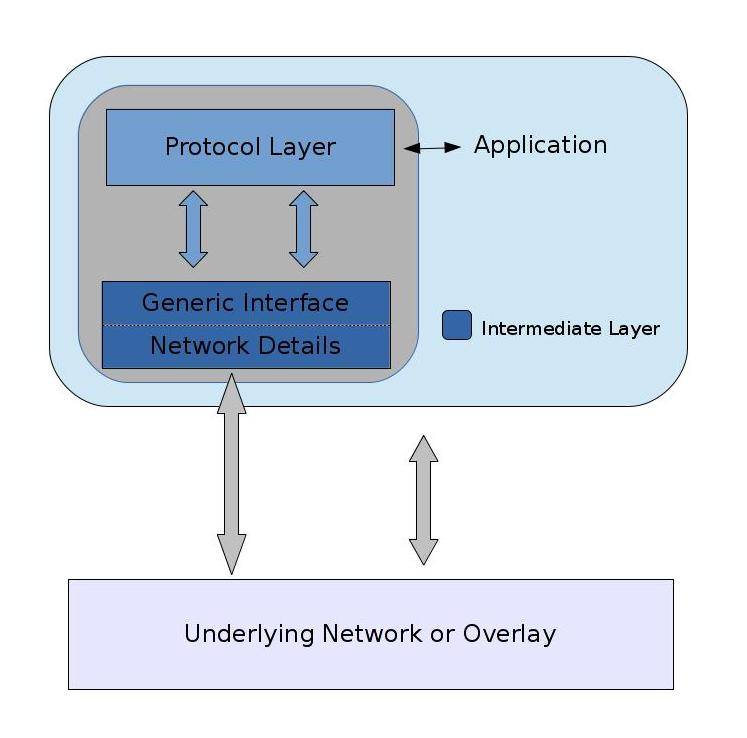
\includegraphics[scale=0.5]{../figures/design_overview.jpg}
	 \caption{The protocol implementation is composed of the components in the gray area. When a global property is required by the application, a request will be sent to the protocol layer. This will be able to make the necessary computations by using the interfaces provided by an intermediate layer, which in turn will contain in a sub-layer all the implementation details for specific underlying networks.}
     \label{fig:design_overview}
\end{figure}


\chapter{Future Plans}
\label{sec:progress}

In this chapter we present the future plans for this project. While the project is still at an early stage we can roughly divide our future work into four main parts.

\subsection*{Protocol Design}

This stage includes familiarization with the underlying decentralized algorithm and the design of the protocol. The resulting protocol should fulfill most if not all of the requirements presented in Chapter \ref{sec:design}. It is important that the proposed protocol will be designed to support both basic and advanced features from the beginning. This means, that the protocol must be designed with extensibility in mind, so that even if some features cannot be implemented due to the time constraints set by the project, adding them in some future work will be trivial. Initially greater emphasis will be given to basic protocol features, such as efficient data exchange of node impulse responses in an asynchronous stable network. More advanced features, such as computing global properties in unstable networks with high churn rates will be part of the second phase of the design, along with possible protocol optimizations. 

\subsection*{Implementation of Basic Functionality}

This will be the first implementation phase, where the basic functionality will be introduced, along with proper interfaces that will allow extending and altering the protocol behavior. Additionally emphasis will be given in minimizing communication costs by finding efficient solutions in sending messages. Finally unit testing will be performed to ensure the correctness of the implementation. Ideally this stage will not come after the protocol design, but will be concurrent, so that implementation issues of the proposed design can be discovered early on and vice versa.

\subsection*{Implementation of Advanced Features}

This phase includes the implementation of the more advanced features. If the design and the initial implementation have been performed correctly, this stage should require less time than the previous. Again communication costs and unit testing will be part of this stage to ensure the quality of the final product.

\subsection*{Testing and Evaluation}

In this stage, further testing of the implemented protocol will be performed to locate and fix major bugs. This testing will also provide a useful and concrete documentation. In addition, the protocol will be evaluated as part of a system that will be built on top of a Pastry overlay network, which will provide very useful information about the efficiency of the proposed protocol and its tolerance to failures. A high level overview of such an evaluation model can be seen in Figure \ref{fig:pastry_evaluation}.

\begin{figure}[!h]
   \centering
     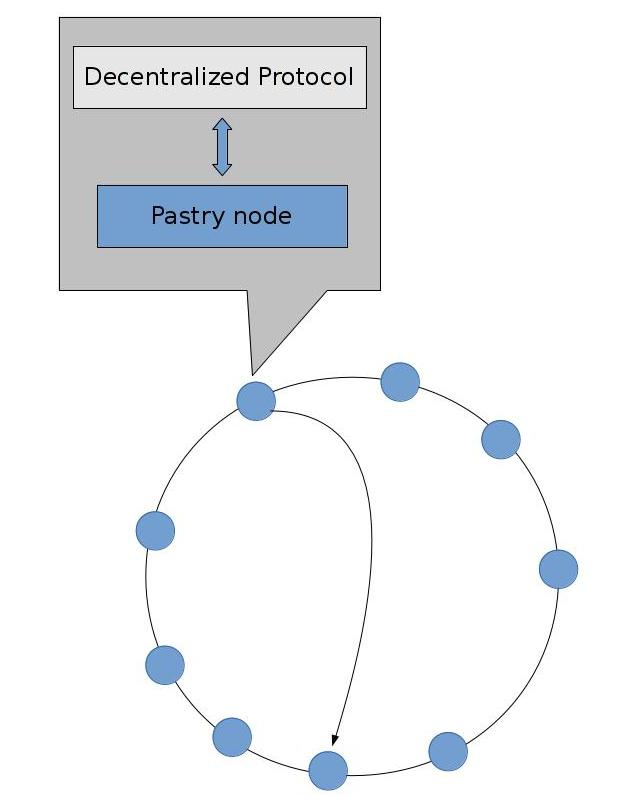
\includegraphics[scale=0.5]{../figures/pastry_evaluation.jpg}
	 \caption{Each node in a pastry overlay network will run our protocol implementation, in order to evaluate its performance}
     \label{fig:pastry_evaluation}
\end{figure}

\subsection*{Consolidating Report and Presentation}

In all of the above stages, the final report will be enriched with all the ideas and approaches that were followed during development. In this stage, the report will be finalized, giving more details into some parts and reaching some conclusions and possible future work. Moreover, the presentation based on the report's findings will be prepared for the final submission.

\bibliography{bibl}
\bibliographystyle{plain}
\end{document}